\documentclass[tikz,border=2mm]{standalone}
\usepackage{tikz}
\usetikzlibrary{matrix,chains,positioning,decorations.pathreplacing,arrows,shadows}
\usetikzlibrary{matrix}
\usetikzlibrary{arrows}
\usetikzlibrary{arrows.meta}
\usetikzlibrary{calc}
\usetikzlibrary{shapes}
\usetikzlibrary{positioning}
\usetikzlibrary{fit}
\usetikzlibrary{intersections}
\usetikzlibrary{decorations.markings}

\begin{document}


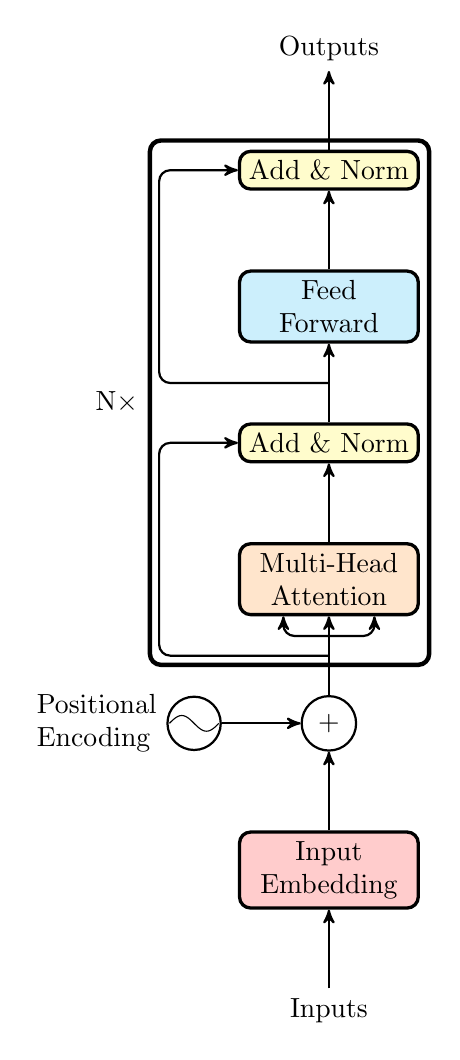
\begin{tikzpicture}[
  module/.style={draw, very thick, rounded corners, minimum width=15ex},
  embmodule/.style={module, fill=red!20},
  mhamodule/.style={module, fill=orange!20},
  lnmodule/.style={module, fill=yellow!20},
  ffnmodule/.style={module, fill=cyan!20},
  arrow/.style={-stealth', thick, rounded corners},
]

  \node (inputs) {Inputs};
  \node[above=of inputs, embmodule, align=center] (inputemb) {Input\\Embedding};
  \node[above=of inputemb, draw, thick, circle] (embplus) {$+$};
  \node[left=of embplus, draw, thick, circle, inner sep=0pt,label={[align=left]left:Positional\\Encoding}] (pe) {\tikz \draw[scale=0.1] plot[domain=0.0:6.28] (\x,{sin(\x r)});};

  \node[above=of embplus, mhamodule, align=center] (mha) {Multi-Head\\Attention};
  \node[above=of mha, lnmodule, align=center] (addnorm1) {Add \& Norm};
  \node[above=of addnorm1, ffnmodule, align=center] (ffn) {Feed\\Forward};
  \node[above=of ffn, lnmodule, align=center] (addnorm2) {Add \& Norm};
  \node[above=of addnorm2] (outputs) {Outputs};

  \coordinate (mharesidual) at ($(mha.south)!0.5!(embplus.north)$);
  \coordinate (ffnresidual) at ($(ffn.south)!0.5!(addnorm1.north)$);
  \coordinate (mhafork) at ($(mha.south)!0.5!(mharesidual)$);
  \coordinate[left=of addnorm1] (ln1residualleft);
  \coordinate[left=of addnorm2] (ln2residualleft);

  \node[fit={(mha)(addnorm2)(mharesidual)(ln1residualleft)}, draw, ultra thick, rounded corners, label=left:$\mathrm{N\times}$] (encoder) {};

  \draw[arrow] (inputs) -- (inputemb);
  \draw[arrow] (inputemb) -- (embplus);
  \draw[arrow] (pe) -- (embplus);
  \draw[arrow] (embplus) -- (mha);
  \draw[arrow] (mha) -- (addnorm1);
  \draw[arrow] (addnorm1) -- (ffn);
  \draw[arrow] (ffn) -- (addnorm2);
  \draw[arrow] (addnorm2) -- (outputs);

  \draw[arrow] (mharesidual)-|(ln1residualleft)--(addnorm1);
  \draw[arrow] (ffnresidual)-|(ln2residualleft)--(addnorm2);
  \draw[arrow] (mhafork)-|($(mha.south)!0.5!(mha.south west)$);
  \draw[arrow] (mhafork)-|($(mha.south)!0.5!(mha.south east)$);
\end{tikzpicture}

\end{document}